\chapter{Framework API}

\section*{\textit{Version 1.0}}

\section{Introduction}

The \class{org.cishell.framework} package and subpackages define the core of
CIShell. The key components being algorithms, data, and CIShell service access.

\subsection{Essentials}
\begin{itemize}
  \item \textit{Application Independence} - Algorithms must be usable in a wide
  variety of contexts and should not be tied to any one CIShell environment or
  front end where possible.
  \item \textit{User Interface Independence} - Algorithms should not have to tie
  themselves to a single UI where possible.
  \item \textit{Black Box Algorithms} - Algorithms are black boxes whose
  possible interactions are described in metadata.
  \item \textit{Delayed Execution} - There may be a large delay between an
  algorithm getting parameters for execution and its actual execution.
  \item \textit{Remote Execution} - Algorithm interfaces should be designed to
  facilitate remote execution of algorithms where possible.
\end{itemize}

\subsection{Entities}

\begin{itemize}
  \item \textit{AlgorithmFactory} - The service interface for algorithms.
  A factory class which creates an \class{Algorithm} for execution from input
  data.
  \item \textit{Algorithm} - The interface for the code execution part of the
  algorithm.
  \item \textit{AlgorithmProperty} - The interface which provides string
  constants for an algorithm's service metadata.
  \item \textit{DataValidator} - The interface an \class{AlgorithmFactory}
  extends to provide additional data validation in addition to the data format validation
  that an application should provide ahead of time.
  \item \textit{ProgressTrackable} - The interface an \class{Algorithm} extends
  to allow for more detailed monitoring and control of an Algorithm's progress while
  executing.
  \item \textit{ProgressMonitor} - The interface for a class to be passed in to
  a \class{ProgressTrackable} \class{Algorithm} so that the \class{Algorithm}
  can be controlled and provide information on its progress while executing.
  \item \textit{Data} - The interface used to pass data (other than
  parameters) and meta-data between algorithms.
  \item \textit{BasicData} - A simple implementation of the \class{Data}
  interface.
  \item \textit{DataProperty} - The interface which provides string constants
  for \class{Data}'s metadata.
  \item \textit{CIShellContext} - The interface for a class to be passed in to
  an \class{AlgorithmFactory} for use in gaining access to standard CIShell
  services.
  \item \textit{LocalCIShellContext} - A simple implementation of the
  \class{CIShellContext} interface which pulls CIShell services from the OSGi
  Service Registry.
\end{itemize}

\begin{figure}[htb!]
\centering
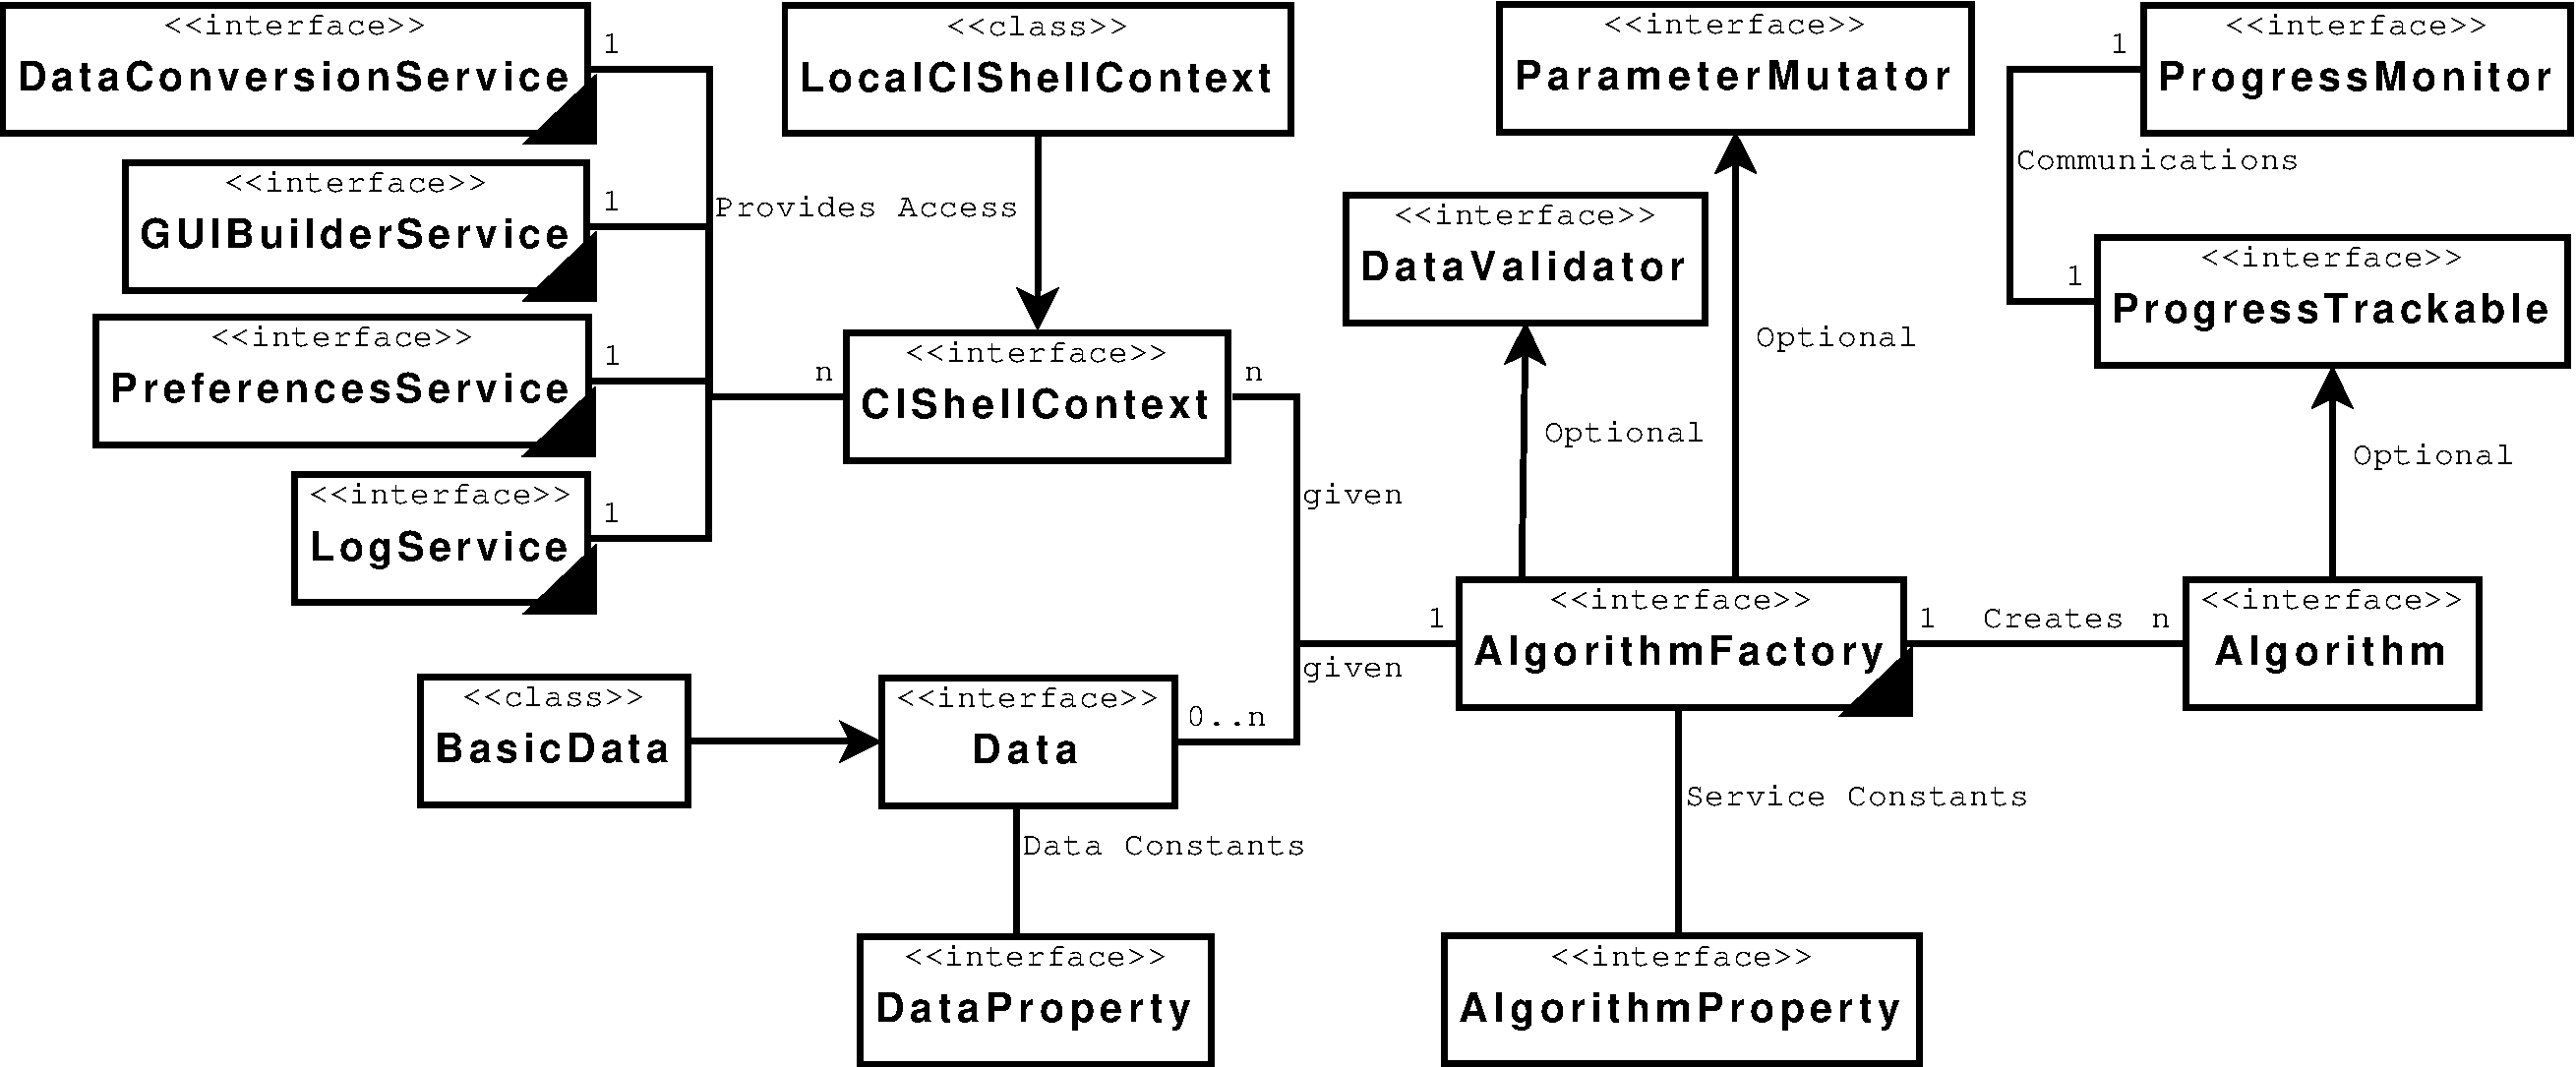
\includegraphics[width=150mm]{../img/cishellInteraction.pdf}
\caption{org.cishell.framework Class Diagram}
\label{fig:cishellInteraction}
\end{figure}

\subsection{Operations}

The algorithm developer should fully implement the \class{AlgorithmFactory}
interface and make it available in OSGi's service registry. The system developer
will provide the services required by CIShell in OSGi's service registry.
Application developers will provide everything else, orchestrating the passing of
information between algorithms.
